\documentclass{beamer}

\usepackage[frenchb]{babel}
\usepackage[T1]{fontenc}
\usepackage[utf8]{inputenc}
\usepackage{amsmath}


\usetheme{Frankfurt}

\title{Compresseur universel}
\author{Noé LE PHILIPPE}
\institute{Université de Montpellier}
\date{\today}
% \logo{\includegraphics[height=10mm]{images/logo.png}}

\addtobeamertemplate{navigation symbols}{}{%
  \usebeamerfont{footline}%
  \usebeamercolor[fg]{footline}%
  \hspace{1em}%
  \insertframenumber/\inserttotalframenumber
}

\AtBeginSection[]
{
  \begin{frame}
    \frametitle{Sommaire}
    \tableofcontents[currentsection, hideothersubsections]
  \end{frame} 
}

\begin{document}

\begin{frame}
  \titlepage
\end{frame}

\section{Structure du compresseur}
\subsection{Compression en deux temps}
\begin{frame}
  \frametitle{Compression d'image}
  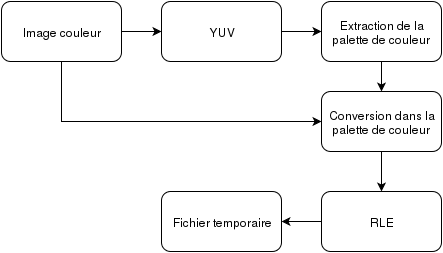
\includegraphics[scale=0.5]{image_compress.png}
\end{frame}
\begin{frame}
  \frametitle{Compression de fichier binaire}
  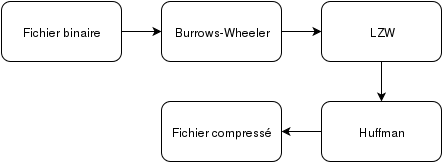
\includegraphics[scale=0.5]{binary_compress.png}
\end{frame}
\section{Détail des méthodes}
\subsection{Extraction de la palette de couleur}
\begin{frame}
  \frametitle{Extraction de la palette de couleur}
  \begin{block}{But}
    Passer de 16 millions (256 * 256 * 256) de couleurs à au maximum 256
  \end{block}
  \begin{block}{Principe}
    Jamais 16 millions de couleurs présentes dans une image
  \end{block}
\end{frame}
\begin{frame}
  \frametitle{Comment extraire la palette}
  \begin{block}{}
    Découpage de l'espace en n zones contenant le même nombre de points
  \end{block}
  \begin{center}
    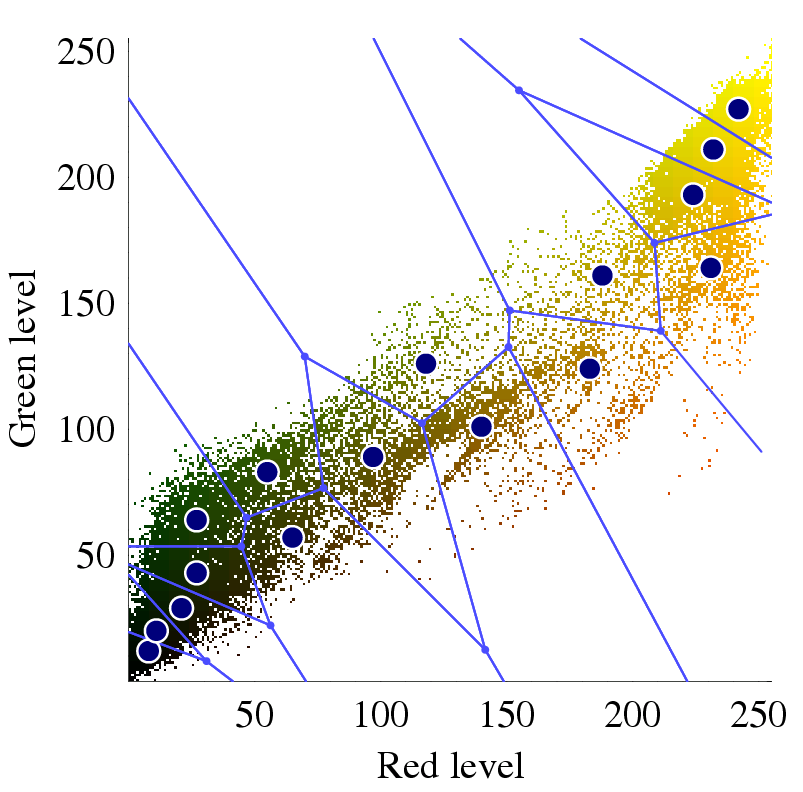
\includegraphics[scale=0.2]{cluster.png}
  \end{center}
\end{frame}
\begin{frame}
  \frametitle{Algorithmes utilisés}
  \begin{block}{YUV}
    Passage de U et V en carrés de 32 * 32
  \end{block}
  \begin{block}{Median-cut}

  \end{block}
  \begin{block}{Kmeans}

  \end{block}
\end{frame}
\subsection{Utilisation de la palette de couleur}
\begin{frame}
  \frametitle{Utilisation de la palette de couleur}
  \begin{block}{Algorithme}
    Pour chaque pixel trouver la couleur dans la palette qui minimise la distance
  \end{block}
  \begin{block}{}
    $$ pixel = min((R_{pix} - R_{pal})^2 + (G_{pix} - G_{pal})^2 + (B_{pix} - B_{pal})^2) $$
  \end{block}
\end{frame}
\subsection{RLE}
  \begin{frame}
    \frametitle{RLE}
    \begin{block}{Efficace}
      Beaucoup de redondances grâce à un espace de couleur réduit
    \end{block}
    \begin{block}{Mise en place}
      1 octet pour le nombre de pixels - 1 octet pour l'indice dans la palette
    \end{block}
  \end{frame}
\section{Codage sans perte}
\subsection{}
\end{document}
